\documentclass{beamer}
\usepackage{ctex,amsmath,tikz,physics,mathrsfs,cite,pgffor}
\usetheme{Madrid}
\usecolortheme{whale}

\renewcommand{\baselinestretch}{1.5}
\setlength{\parindent}{2em}
\definecolor{pureblue}{rgb}{0,0,1}
\hypersetup{citecolor=pureblue}%文献引用颜色
\bibliographystyle{plain}

\title{Ghost Hunter Design Report}
\author{Team wyy:\ 武益阳\ 王宇逸}
\date{\today}

\begin{document}
\begin{frame}
    \titlepage
\end{frame}

\begin{frame}
    \frametitle{Contents}
    \tableofcontents
\end{frame}

\section{Idea}
\begin{frame}
    \frametitle{Idea}
    \large
    \begin{enumerate}
        \item Threshold method can precisely and easily find at least the first PE. \pause
        \item Waveform of several PEs is the supersposition of single waveform of these PEs. \pause
    \end{enumerate}
    
    So, use threshold method to find the first PE and substract single PE waveform from original waveform, in order to search for the next PE.
\end{frame}

\section{Find Single PE Waveform}
\begin{frame}
    \frametitle{Find Single PE Waveform}
    \large
    \begin{enumerate}
        \item Select waveform whose PE numbers = 1. \pause
        \item Use cuts to ensure that signal is within the range and not to weak. \pause
        \item According to \cite{ref1}, the standard waveform for a single PE is:\\
        \begin{equation*}
        \begin{array}{ll}{0 \leq t<T :} & {i_{i n}(t)=I_{s}\left(1-e^{-t / R C}\right)} \\ {T \leq t \leq \infty} & {i_{i n}(t)=I_{s}\left(e^{T / R C}-1\right) \cdot e^{-t / R C}}\end{array}
        \end{equation*}
    \end{enumerate}
\end{frame}

\begin{frame}
    \frametitle{Find Single PE Waveform}
    \large
    Fit single PE waveform with function
    \begin{equation*}
        \begin{array}{ll}{T_1 \leqslant t<T_2 :} & U=A\left(1-e^{-t / R C}\right) \\ {t\geqslant T_2:} & U=A\left[e^{(T_2-T_1) / R C}-1\right] e^{-t / R C}\end{array}
    \end{equation*}
    
    \begin{tikzpicture}
        \centering
        % 引入图片
        \node[anchor=south west,inner sep=0] (image) at (0,0) {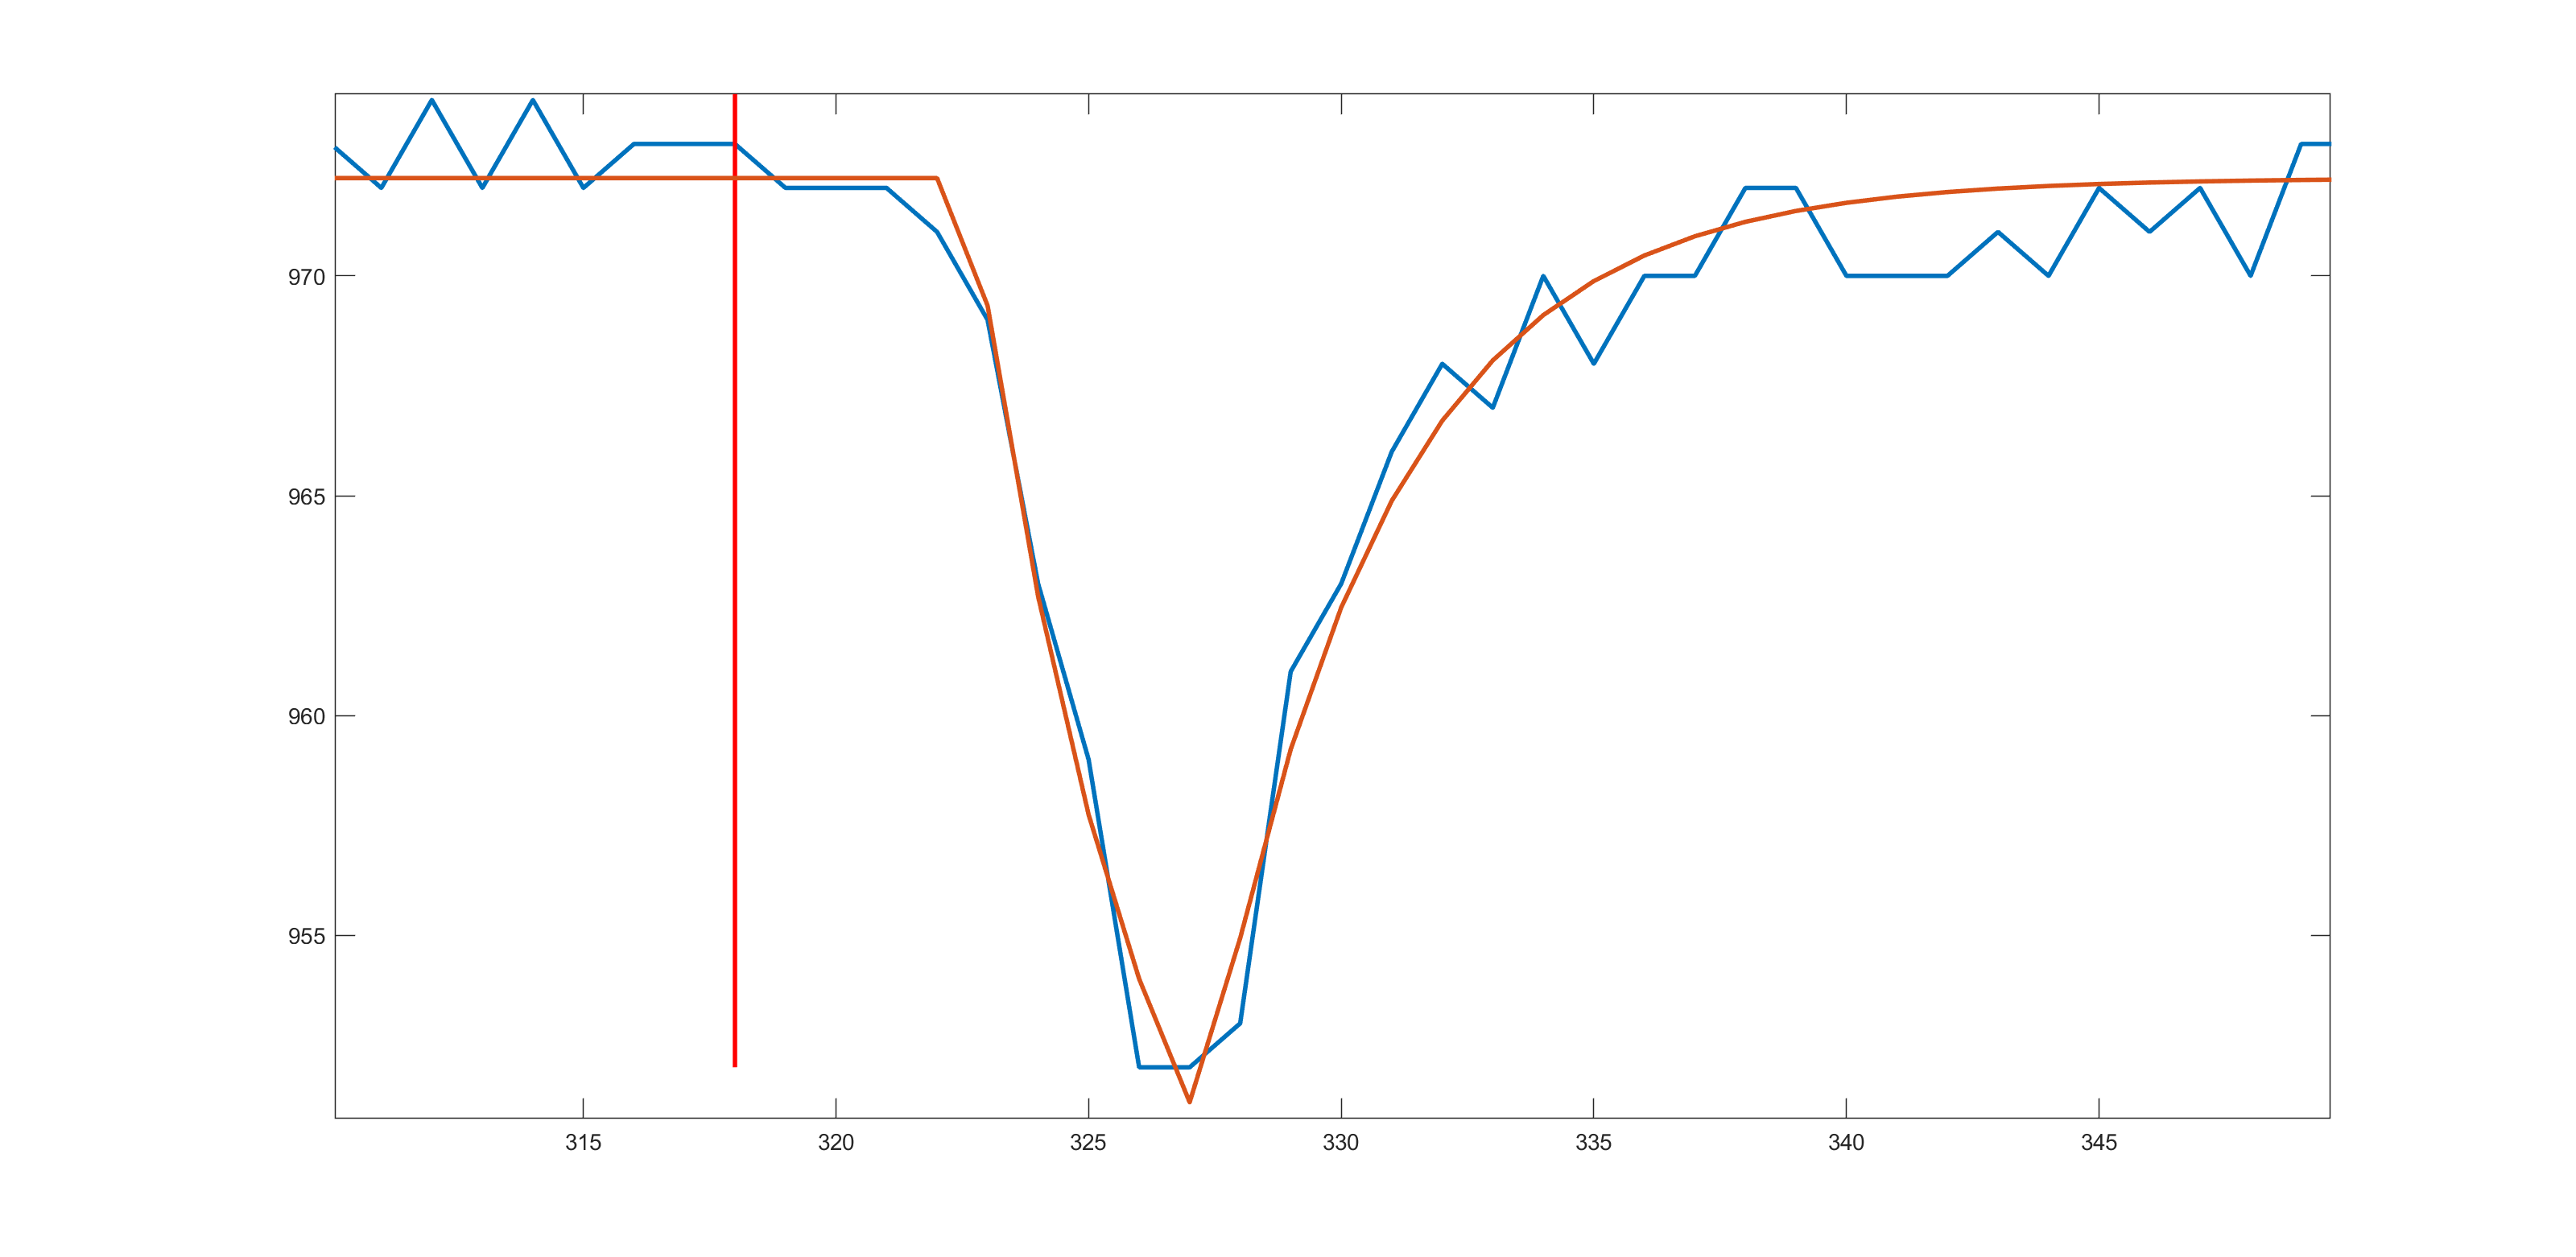
\includegraphics[width=0.6\textwidth]{fig1.png}};
            \begin{scope}[x={(image.south east)},y={(image.north west)}]
                % 建立相对坐标系
                % \draw[help lines,xstep=.1,ystep=.1] (0,0) grid (1,1);
                % \foreach \x in {0,1,...,9} { \node [anchor=north] at (\x/10,0) {0.\x}; }
                % \foreach \y in {0,1,...,9} { \node [anchor=east] at (0,\y/10) {0.\y}; }
                % 作图命令
                \onslide<2->{
                \draw[red,thick,<->] (0.285,0.9) -- (0.37,0.9);
                \node at (0.33,0.96) {$T_1$} ;
                }
                \onslide<3->{
                \draw[red,thick,<->] (0.285,0.12) -- (0.46,0.12);
                \node at (0.38,0.18) {$T_2$} ;
                }
            \end{scope}
    \end{tikzpicture}
\end{frame}

\begin{frame}
    \frametitle{Fit Results}
    \centering
    \large
    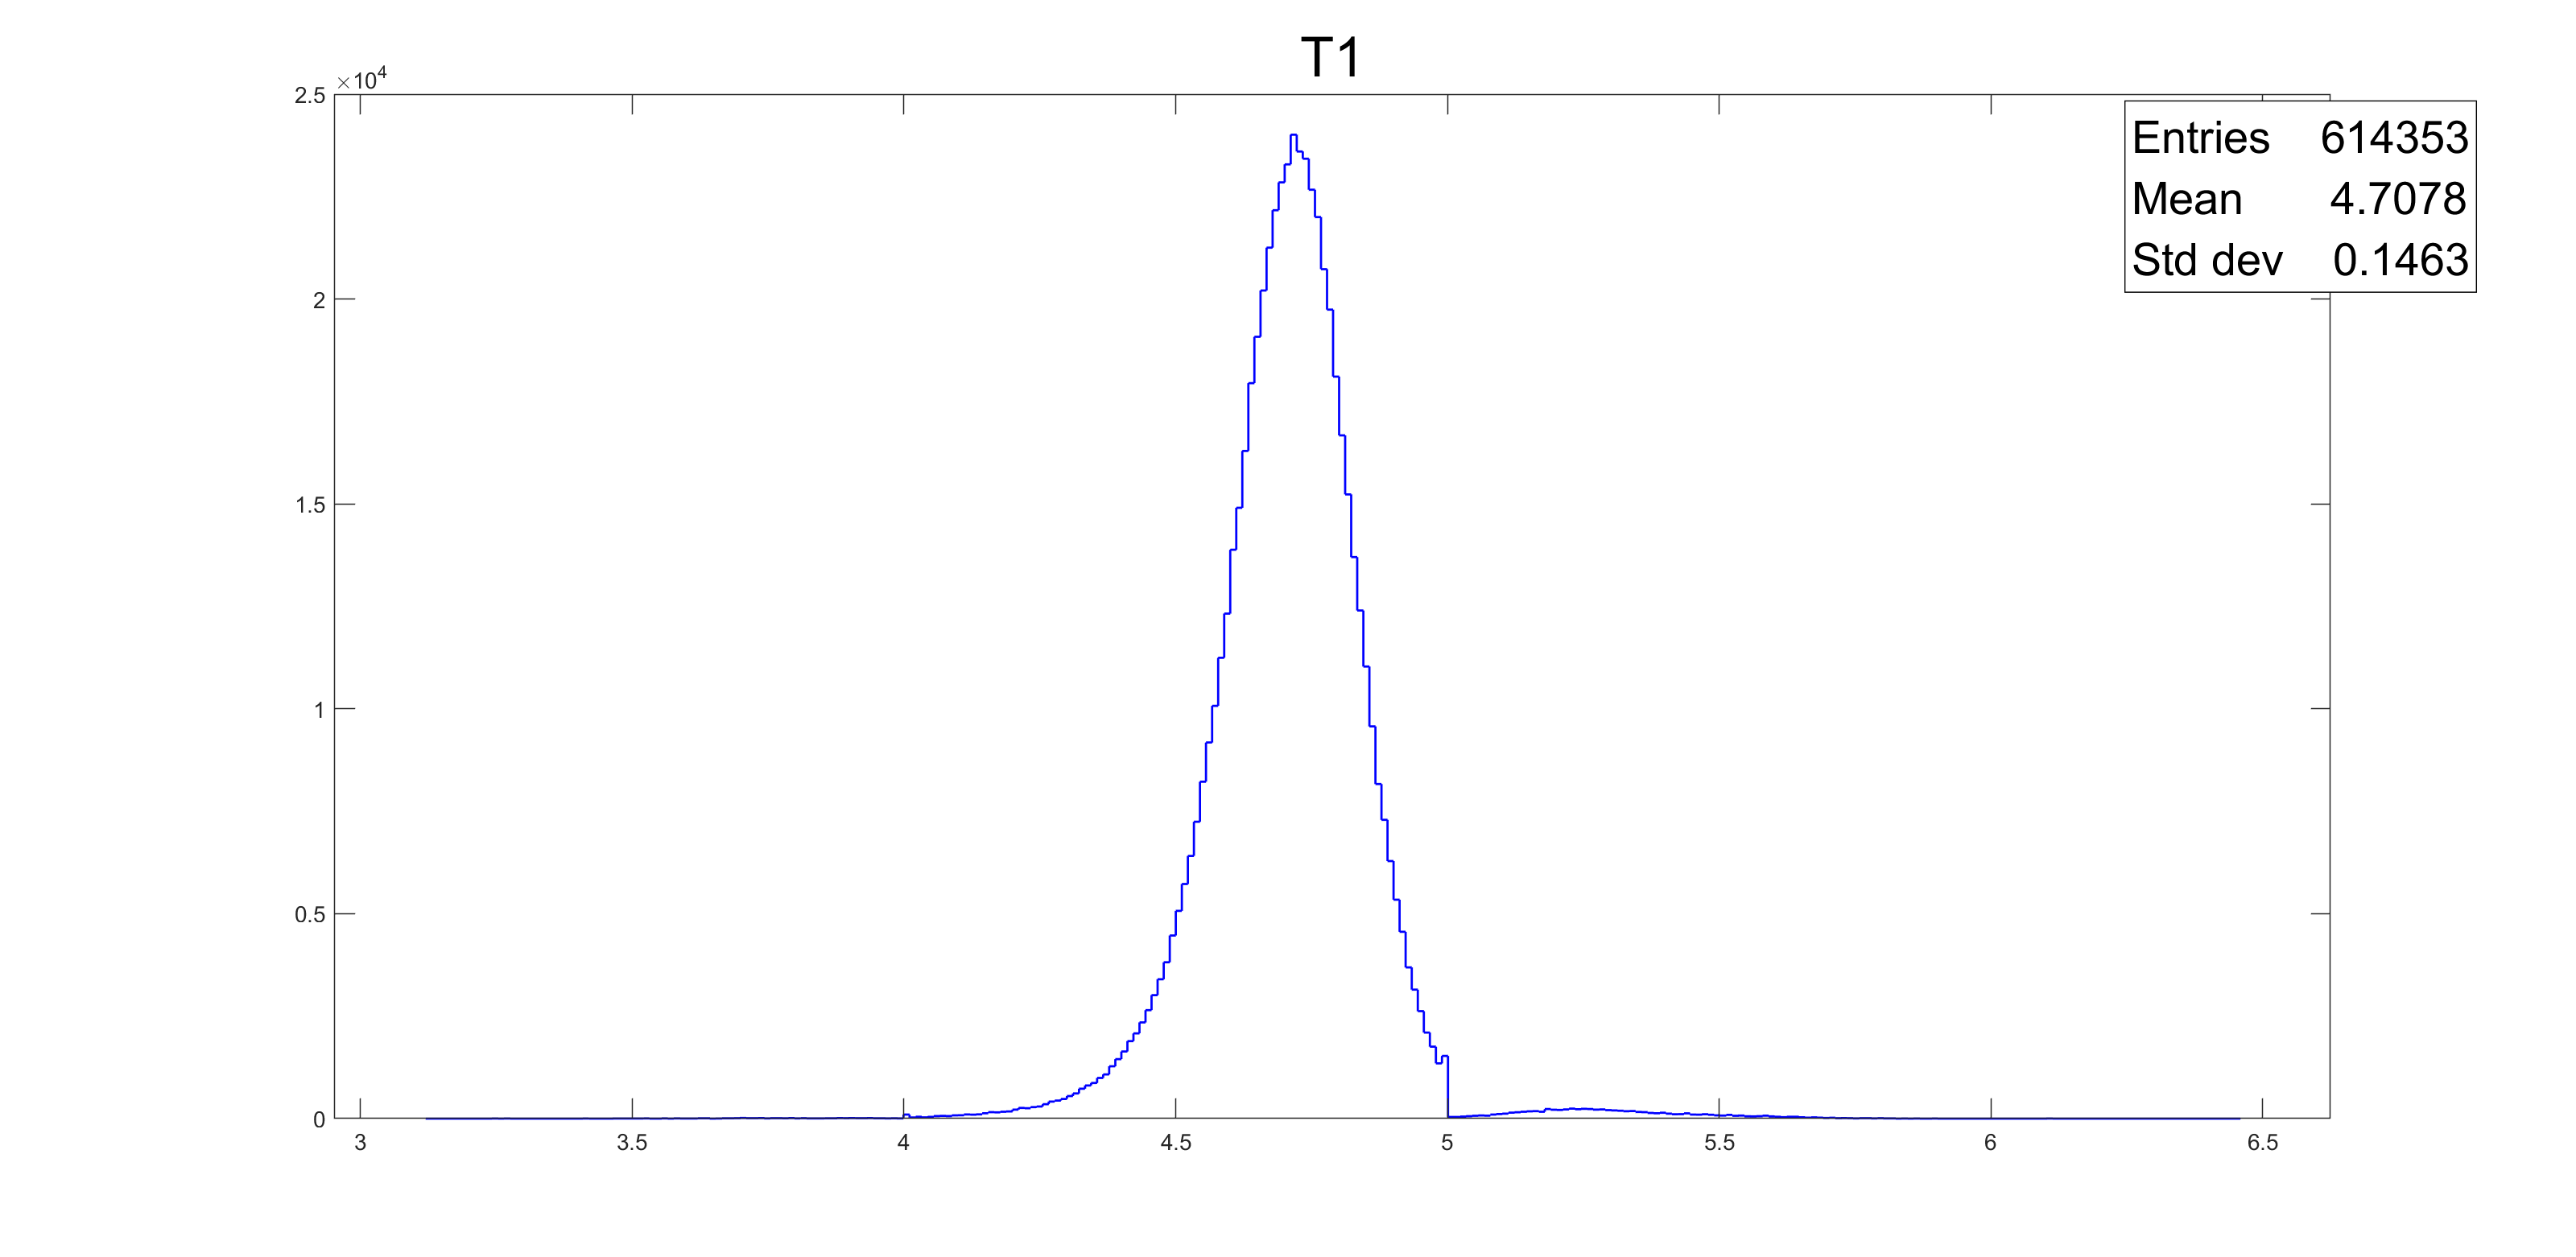
\includegraphics[width=\textwidth]{h1.png}
\end{frame}
\begin{frame}
    \frametitle{Fit Results}
    \centering
    \large
    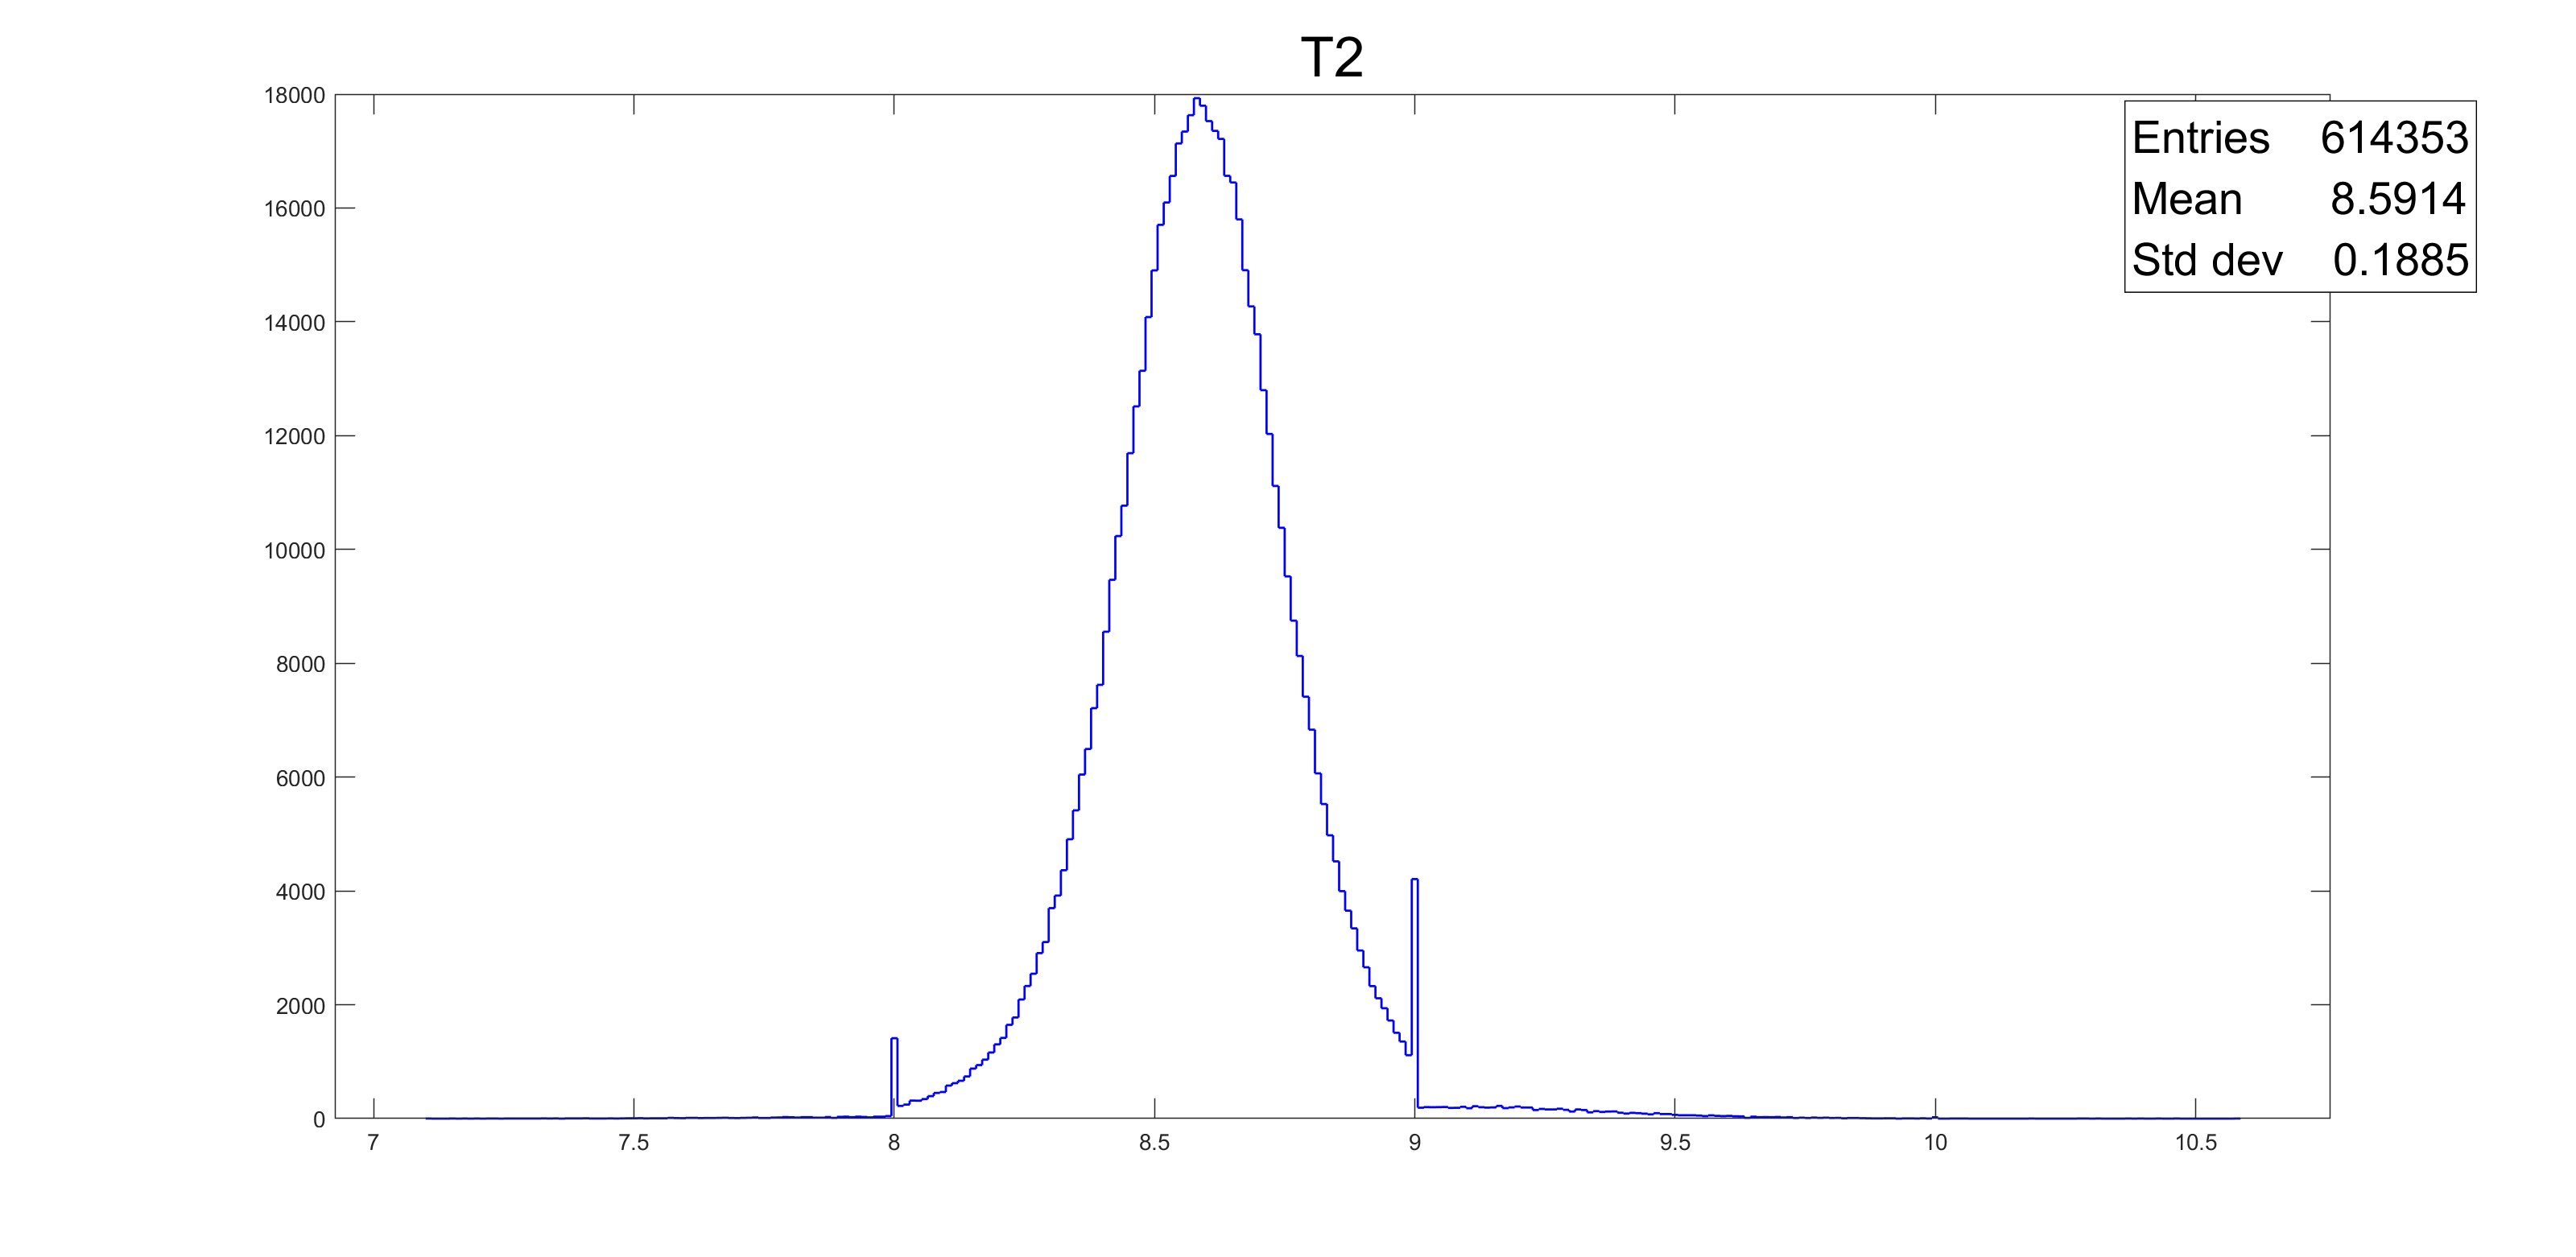
\includegraphics[width=\textwidth]{h2.png}
\end{frame}
\begin{frame}
    \frametitle{Fit Results}
    \centering
    \large
    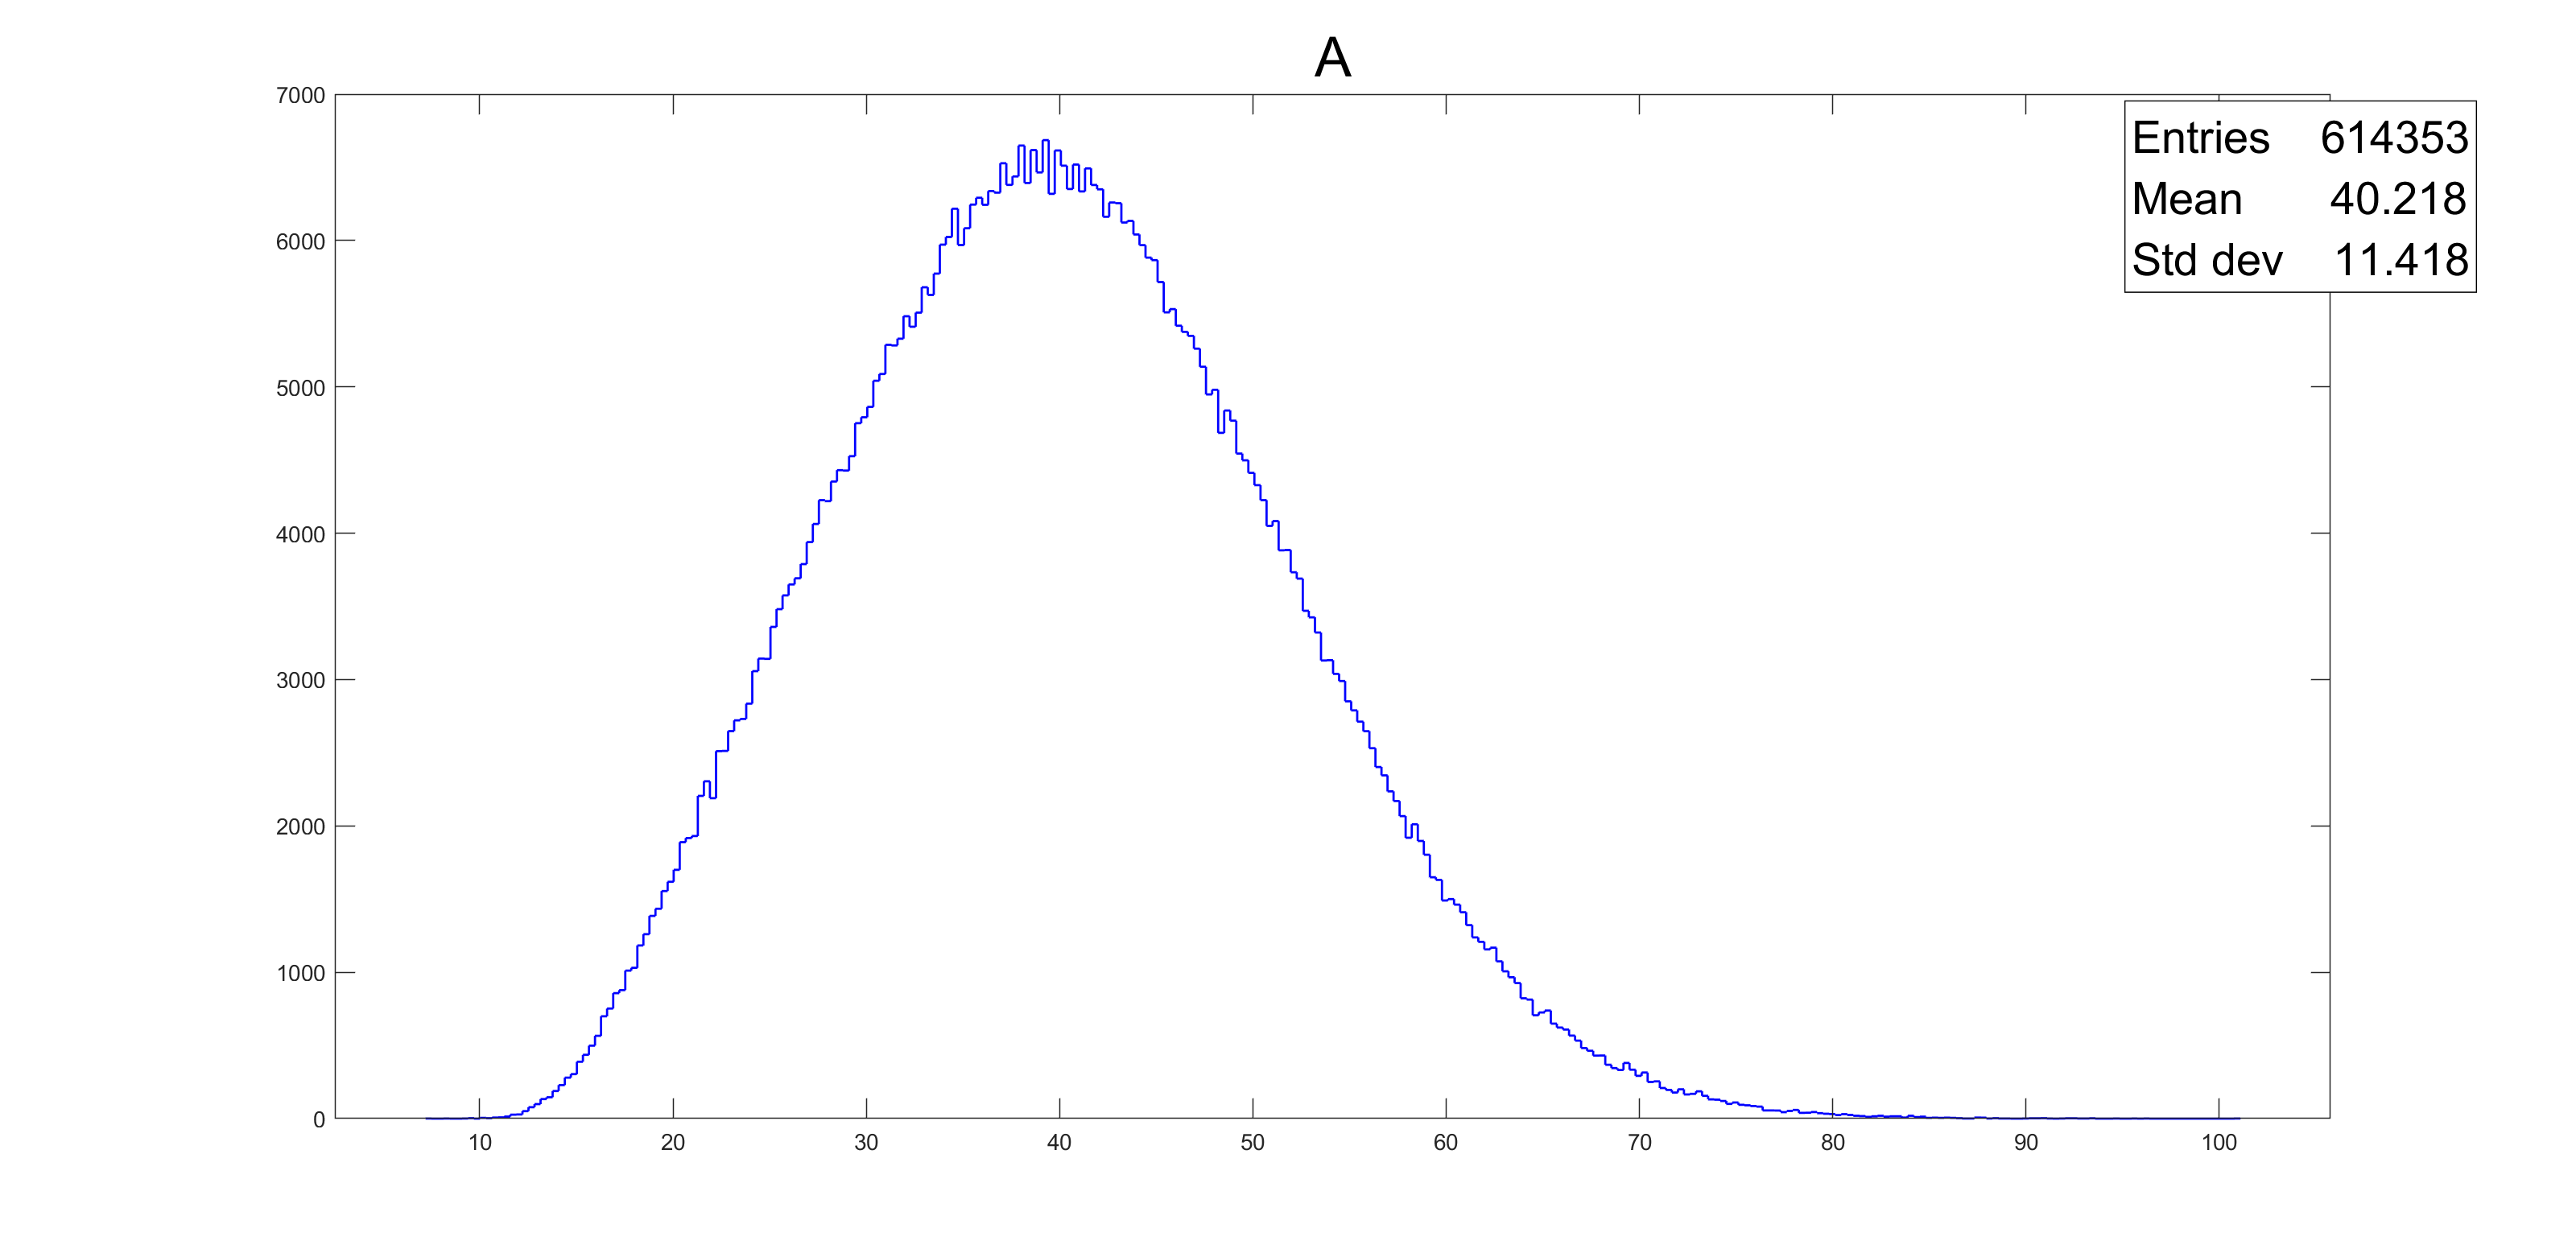
\includegraphics[width=\textwidth]{h3.png}
\end{frame}
\begin{frame}
    \frametitle{Fit Results}
    \centering
    \large
    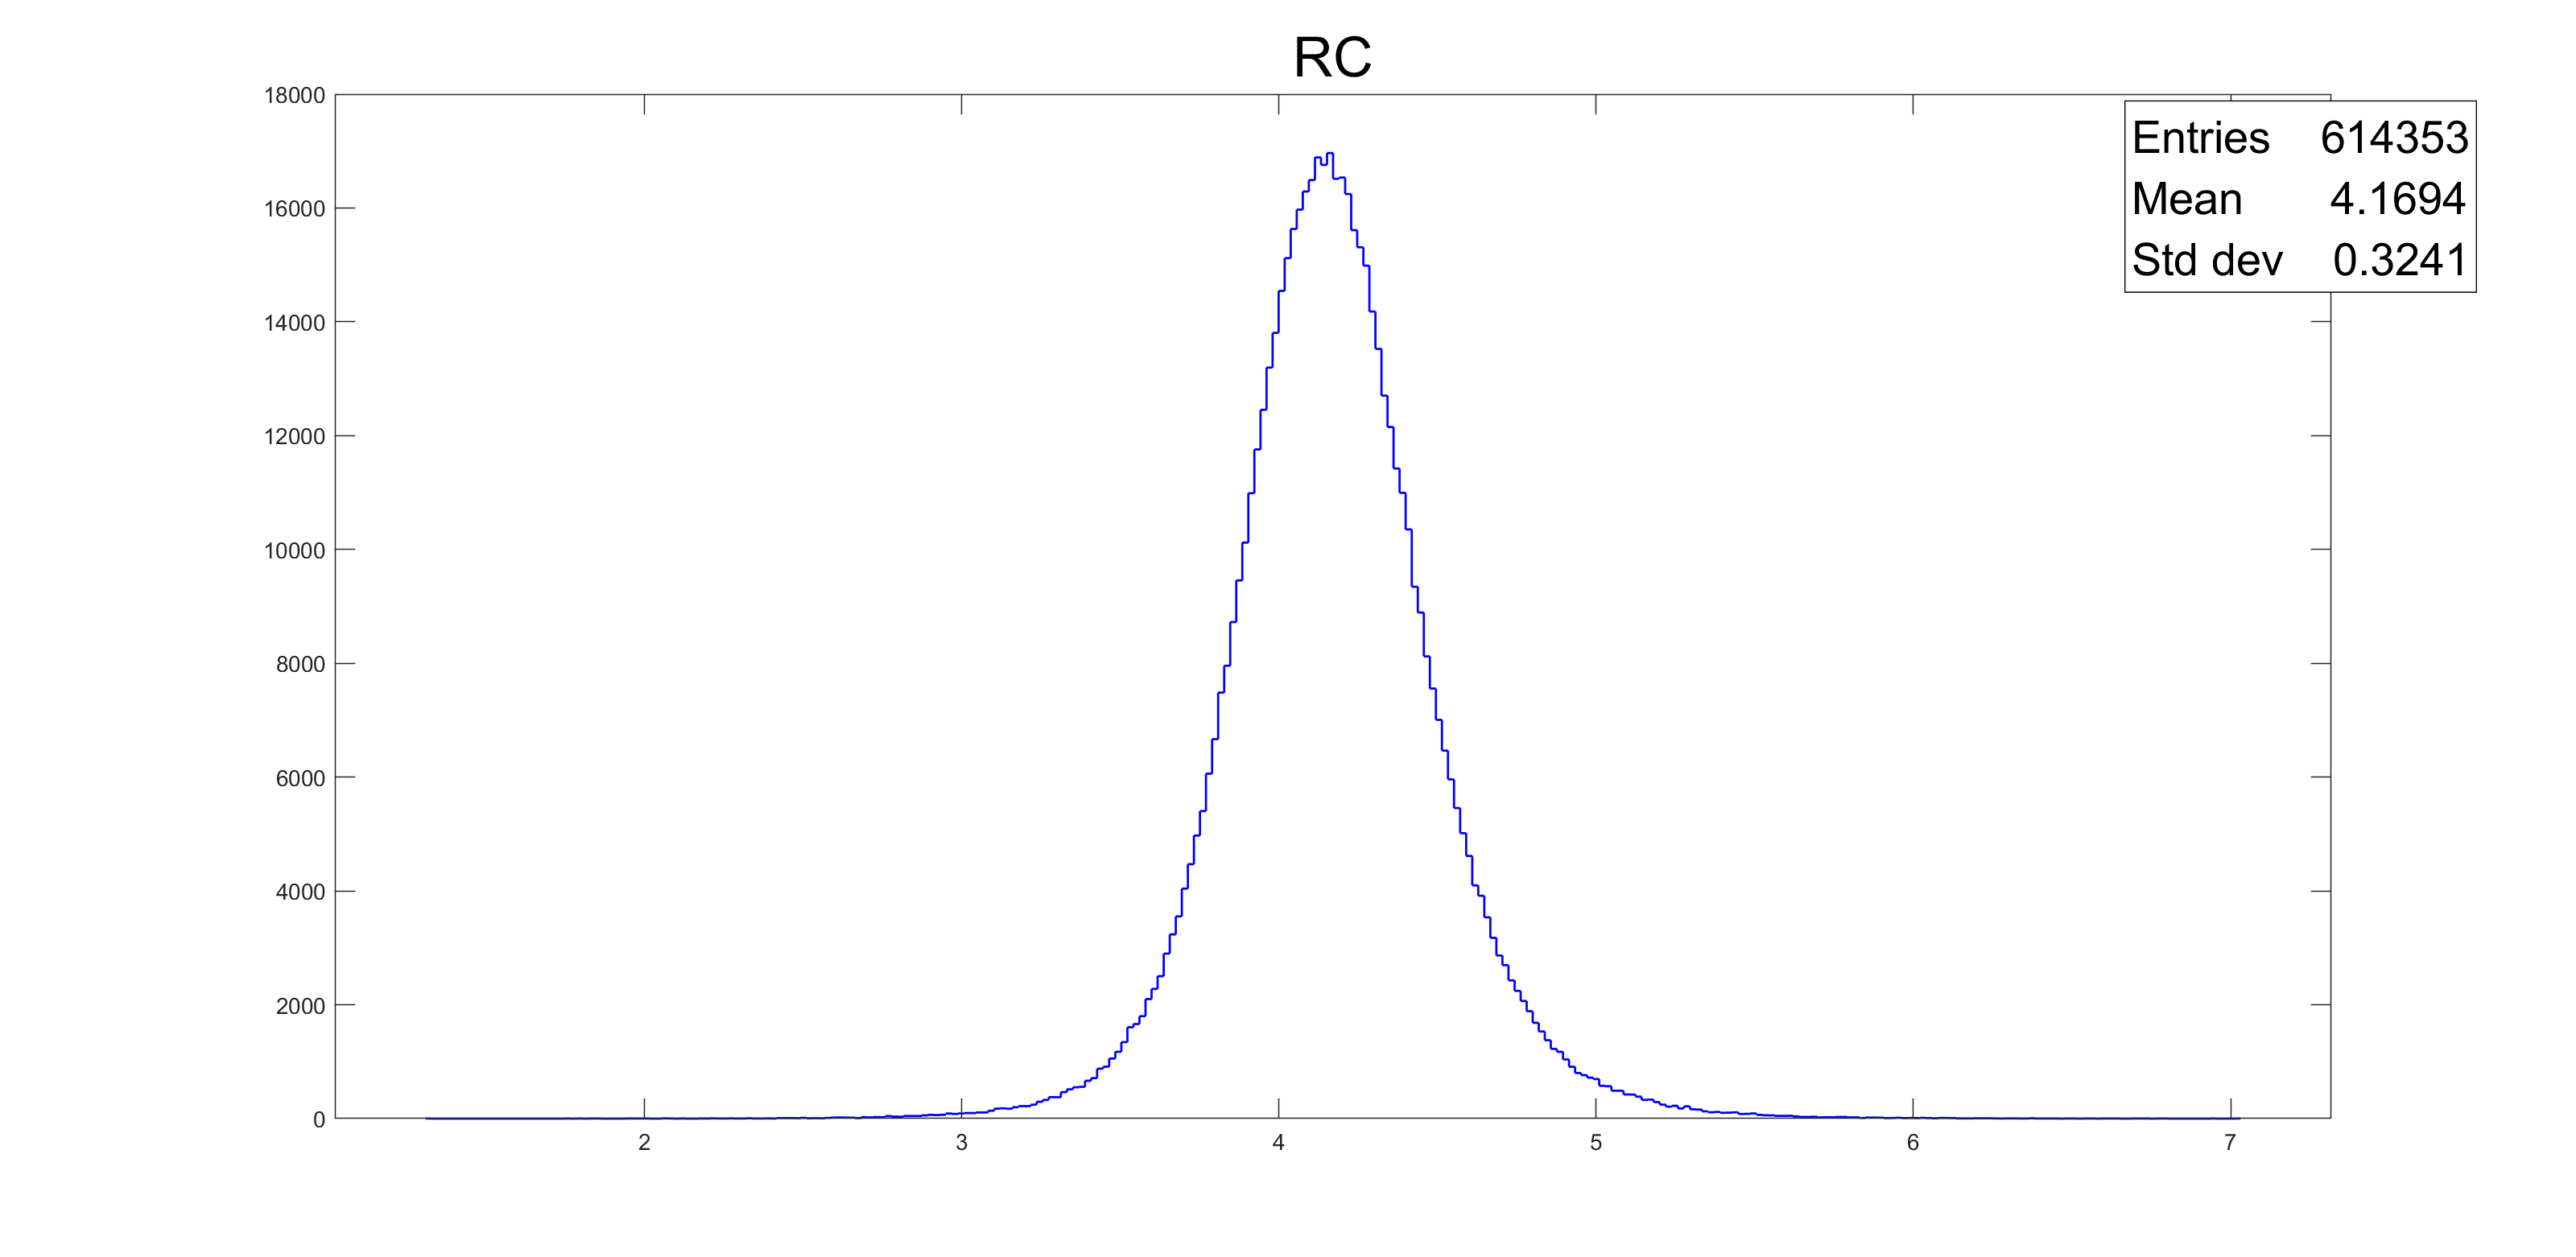
\includegraphics[width=\textwidth]{h4.png}
\end{frame}

\section{Process}
    \foreach \i in {1,...,7}{%
    \begin{frame}
        \frametitle{Process}
        \centering
        \includegraphics[width=0.9\textwidth]{picset1/(\i).png}
    \end{frame}
}

\begin{frame}
    \frametitle{Process}
    \large
    answer: 288,291,309,324,326,331,342\\
    truth : 288,291,309,324,325,329,342\\
    wasserstein\_distance = 0.4286\\
\end{frame}

\begin{frame}
    \frametitle{Exceptions}
    \large
    \begin{itemize}
        \item Tiny signals. \pause
        \item Sigals in the beginging or the end. \pause
        \item Some single-PE waves does not fit well (especially the descending part) $\Rightarrow$ tail after substracting $\Rightarrow$ fake PE found. \pause
    \end{itemize}
    Solution: process exceptional signals separatedly; cut fake PEs.
\end{frame}

\begin{frame}
    \frametitle{\ }
    \Huge
    \centering
    Thanks for listening!
\end{frame}

\section{Reference}
\begin{frame}
    \frametitle{Reference}
    \large
    \bibliography{report.bib}
\end{frame}
\end{document}